% There was a beginning and there was an end. The end.

% \newcommand*\lined[1]{\bar{#1}}
\subsubsection{Introduction}
In \cite{Secord:2002} by Adrian Secord a set of \textit{techniques for generating stipple drawings from grayscale images using weighted centroidal Voronoi diagrams as in the traditional artistic technique of stippling that places small dots of ink onto paper such that their density give the impression of tone.} 

This document describes a replication of the implementations in\cite{Secord:2002} by Adrian Secord. This paper describes a set of techniques for generating stipple drawings using weighted centroidal voronoi diagrams. It also describes several optimization techniques for better performance but a loss in detail. This document is part of a replication study wherein python code is written in - accordance with the original paper. 

\subsubsection{Methods}
The original paper refers to OpenGL for gpu acceleration. Due to complexity reasons this has been left out of this implementation. Python has been used as the programming language. To generate the Voronoi diagrams, the \href{http://www.overleaf.com}{Scipy Voronoi} package has been used which uses the widely used \href{http://www.qhull.org/}{Qhull library}. The code has been written in a Jupyter notebook for easy access. As the Scipy Voronoi library does not deal with boundaries, code has been used that deals with this issue\cite{stackoverflow:2016}. A special requirement in this implementation is that images have to be rectangular.

% Three years, we launched ReScience, a new scientific journal aimed at publishing the
% replication of existing computational research. Since ReScience published its first
% article\supercite{Topalidou:2015}, things have been
% going steadily. We are still alive, independent and without a budget. In the
% meantime, we have published around 24 articles (mostly in computational
% neuroscience \& computational ecology) and the initial
% \href{https://rescience-c.github.io/board/}{editorial board} has grown from
% around 10 to roughly 100 members (editors and reviewers), we have advertised
% ReScience at several conferences worldwide, gave some
% interviews\supercite{Science:2018}, and published an article introducing
% ReScience in PeerJ~CS\supercite{Rougier:2017}. Based on our
% experience\supercite{Rougier:2018} at managing the journal during these three
% years, we think that time is ripe for some changes.



\subsubsection{Voronoi diagrams}
As the introduction suggests, the stipples are created by using voronoi diagrams. Thus it is important that voronoi diagrams are understood first. Imagine a two dimensional plane\(p\). On this plane \(p\) there is a set \(\P\) containing points denoted as \(x\). These points are defined by their x,y components on the plane. 

\begin{figure}
\centerline{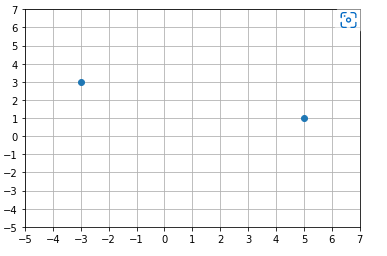
\includegraphics{images/plane_p.png}}
\caption{A top down view of plane p with points \(x_1, x_2\). The plane can be infinite.\newline}
\label{figPlaneP}

 A voronoi diagram splits this plane into \(n\) regions \(A\) where \(n\) is equal to the amount of points \(x\), so that all imaginary points in region \(A_n\), are always closest to the 'real' point in region \(A_n\). This is done by creating a line from point x1 to x2. Then on the midpoint of that line between \(x_1, x_2\); create a new line perpendicular to the first. The new line divides all points on the plan into two regions \(A_1, A_2\). See \ref{figPlanePDivider} for the result.
 
 Creating a line perpendicular to line \(\overline{x_1 x_2}\) is done by creating a two dimensional matrix containing the x,y components and then transforming them:\newline\newline
 \( \begin{bmatrix}x_1x & x_1y\\x_2x & x_2y\end{bmatrix}\rightarrow\begin{bmatrix}-x_1y & x_1x\\-x_2y & x_2x\end{bmatrix}\)\newline\newline
 The perpendicular line then only has to be set to the correct coordinates in the plane equal to the midsection of \(\overline{x_1 x_2}\)

\centerline{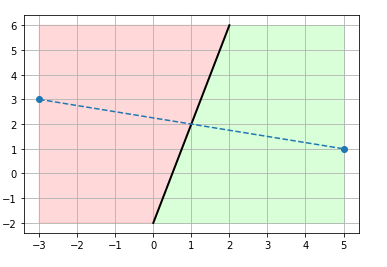
\includegraphics{images/plane_division.png}}
\caption{Dividing line separating the plane into two regions. Each of these regions defines an area wherein all points in that area are closer to either \(x_1\) or \(x_2\). All points on the line are equilateral distance from \(x_1, x_2\)}
\label{figPlanePDivider}
\end{figure}

\begin{figure}
\centerline{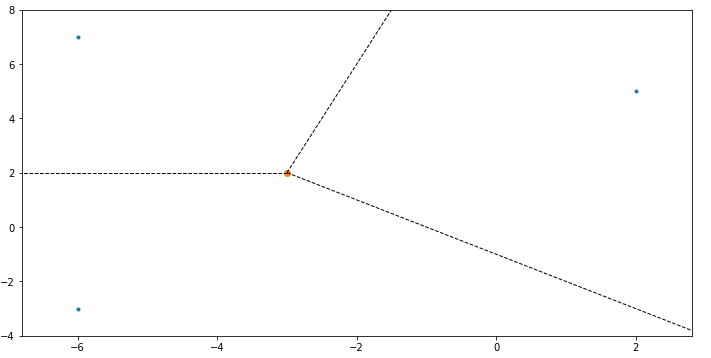
\includegraphics{images/plane_p_3.png}}
\caption{Example with three points in a Voronoi diagram.\newline}
\label{figPlaneP}
\end{figure}

% \clearpage

\let\Oldsection\section
\renewcommand{\section}{\FloatBarrier\Oldsection}

\let\Oldsubsection\subsection
\renewcommand{\subsection}{\FloatBarrier\Oldsubsection}

\let\Oldsubsubsection\subsubsection
\renewcommand{\subsubsection}{\FloatBarrier\Oldsubsubsection}
\subsubsection{Centroidal Voronoi diagrams}
To go from voronoi diagrams to visually pleasing stippling images it is imperative to use some weighting function. A voronoi diagram splits a plane - such as an image - into \(n\) regions \(A\). To determine where stipples should be placed a weighting function is used. The weighting function is applied to every region and is used to move the point inside each region to it's most average position based on. The weighting function takes the intensity of every pixel inside of a region and determines where the average intensity point in a region is. It then moves the real point in that region to the weighted function point. it does so for every 'real' point on the plane iteratively until all points are in their centroidal location within their regions.

The centroid of a region is defined as: \(C_i = \frac{\int_A \pmb{x}p(\pmb{x})dA)}{\int_A p(\pmb{x})dA}\)\newline
\(A\) is the region, \(\pmb{x}\) is the position and \(p(\pmb{x})\) is the density\cite{Secord:2002}.\newline

\subsubsection{Generating Voronoi diagrams}
Matplotlib has a voronoi module. Using this implementation has two major advantages:

\begin{itemize}
  \item The code is fully functional and widely supported;
  \item The vertices belonging to a region are clockwise ordered, this is a requirement for the scan-line implementation later on.
\end{itemize}

\label{DensityFunctionSection}
\subsubsection{Density function}
Now that there is an understanding of how Centroidal Voronoi diagrams work, a function is required that generates the initial starting points using a density function. The density function will generate a map of points where darker regions will have more points and lighter regions fewer points. Rejection sampling was used to generate points over our intensity pixel distribution. All greyscale pixels are first converted into a scale (0 < v < 1) where 1 is white and 0 black. Then three vectors are generated with n length using a uniform distribution function. The first two vectors are used to access pixel (x,y) data. The intensity of each pixel is then compared to the probability value. If it is greater than P(x) it is added to the list of starting regions. 

\begin{figure}[!htb]
\centerline{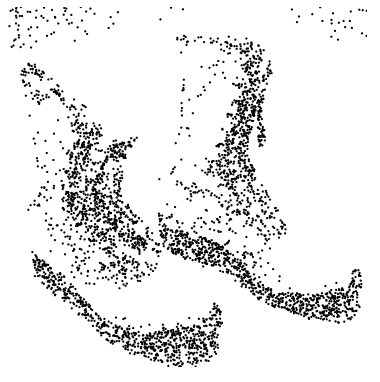
\includegraphics{images/uniform_distribution_shoes.png}}
\caption{Initial points from the density function using a uniform distribution\newline}
\label{figPlaneP}
\end{figure}

By using  different distribution functions, it is possible to 'preserve detail' in some areas of the image. Currently a uniform distribution is being used but with a normal (gaussian) distribution the center of the image would be weighted heavier than the boundaries - resulting in more detail (stipples) in the center.

\subsubsection{Generating stippling image}
Using the result of the density function as our initial input. These are then used to iteratively generate centroidal voronoi diagrams until the average sum of the points update is less than some value. \(\frac{\sum_{i=1}^{Gp} | old_i - new_i |}{Gp} < o\) where \(o\) is the convergence value and \(Gp\) the amount of points.

\begin{figure}[!htb]
\begin{subfigure}[h]{0.4\linewidth}
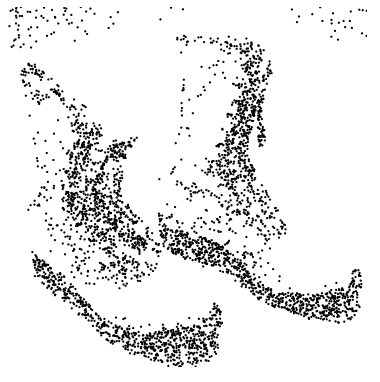
\includegraphics[width=\linewidth]{images/uniform_distribution_shoes.png}
\caption{Uniform distribution generation}
\label{comparison-a}
\end{subfigure}
\hfill
\begin{subfigure}[h]{0.4\linewidth}
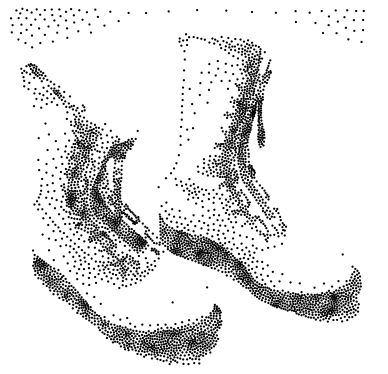
\includegraphics[width=\linewidth]{images/voronoi_stippledshoes.png}
\caption{Centroidal Voronoi distribution}
\end{subfigure}%
\caption{Difference between a hobbyist and an experienced professional}
\label{comparison}
\end{figure}

There is a distinct difference between the initial starting positions and after running the Voronoi algorithm until it has converged. In Figure \ref{comparison-a} it is already clearly visible what the final output image will look like - just a lot grainier. This adds the benefit that options can be tweaked before running the Voronoi stippling to adjust things such as pixel intensity threshold\footnote{This threshold can be set to a level between \(0 < intensity < 255\). The lower it is the more the algorithm will focus on darker regions}, resolution of the image and amount of stipple points to generate.

\label{precompute-stipple-levels}
\subsubsection{Precomputing stipple levels}
The solution mentioned in section\ref{DensityFunctionSection} can be slow. A faster implementation is mentioned in the original paper\cite{Topalidou:2015}. By precomputing a range of stipple levels and applying these to the image a faster version can be created that computes a stipple image in \(O(n)\)  time where \(n\)  is the amount pixels.  

\begin{figure}[!htb]
\begin{subfigure}[h]{0.4\linewidth}
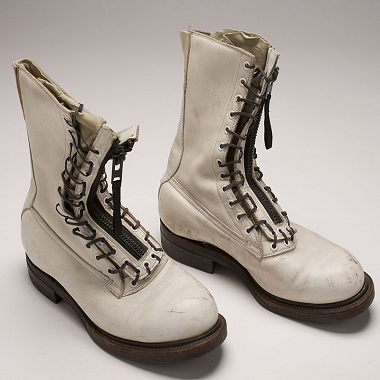
\includegraphics[width=\linewidth]{images/boots_square_380.png}
\caption{Original (input) image}
\label{comparison-a}
\end{subfigure}
\hfill
\begin{subfigure}[h]{0.4\linewidth}
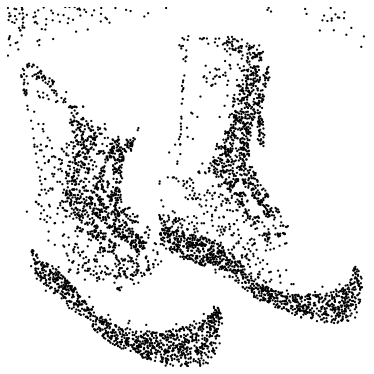
\includegraphics[width=\linewidth]{images/voronoi_shoes_distribution_stipples.png}
\caption{Initial points}
\end{subfigure}%

\begin{subfigure}[h]{0.4\linewidth}
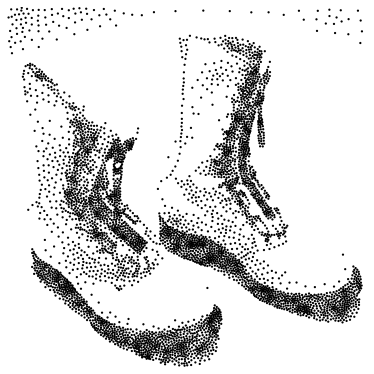
\includegraphics[width=\linewidth]{images/voronoi_shoes_default_stipples.png}
\caption{Default Voronoi stipples generation}
\end{subfigure}%
\hfill
\begin{subfigure}[h]{0.4\linewidth}
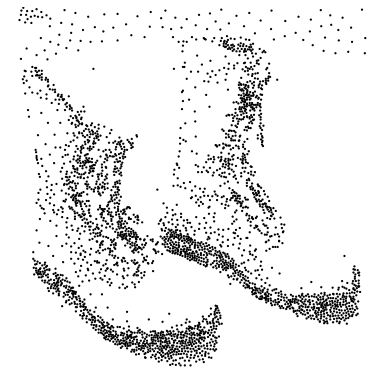
\includegraphics[width=\linewidth]{images/voronoi_shoes_fast_stipples.png}
\caption{Fast Voronoi stipples generation}
\end{subfigure}%
\caption{Comparison between the default (slow) detailed implementation and fast implementation}
\label{comparison-fast}
\end{figure}

\subsubsection{Results}
The implementation yields similar visual results to those found in the original paper. Unfortunately no GPU with OpenGL support is available in this version. 

The fast stippling method results in images similar in quality to the initial distribution\ref{comparison-fast}. The original paper does not offer a visualization of the initial distrubitions making it difficult to compare with the original results. Several configurations have been tried and tested for the fast voronoi stippling method but the results were quite similar. 

\begin{figure}[!htb]
\begin{subfigure}[h]{0.4\linewidth}
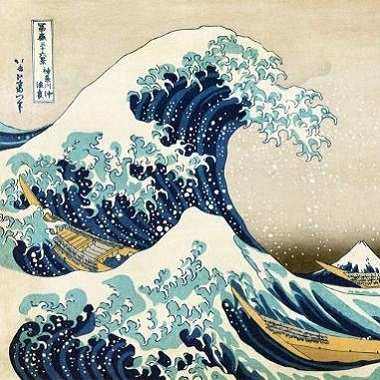
\includegraphics[width=\linewidth]{images/gw_square.jpg}
\caption{Original image (waves)}
\label{comparison-a}
\end{subfigure}
\hfill
\begin{subfigure}[h]{0.4\linewidth}
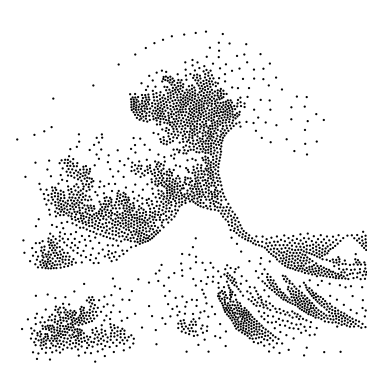
\includegraphics[width=\linewidth]{images/voronoi_wave_default_stipples.png}
\caption{Stippled waves (5000 stipples)}
\end{subfigure}%

\begin{subfigure}[h]{0.4\linewidth}
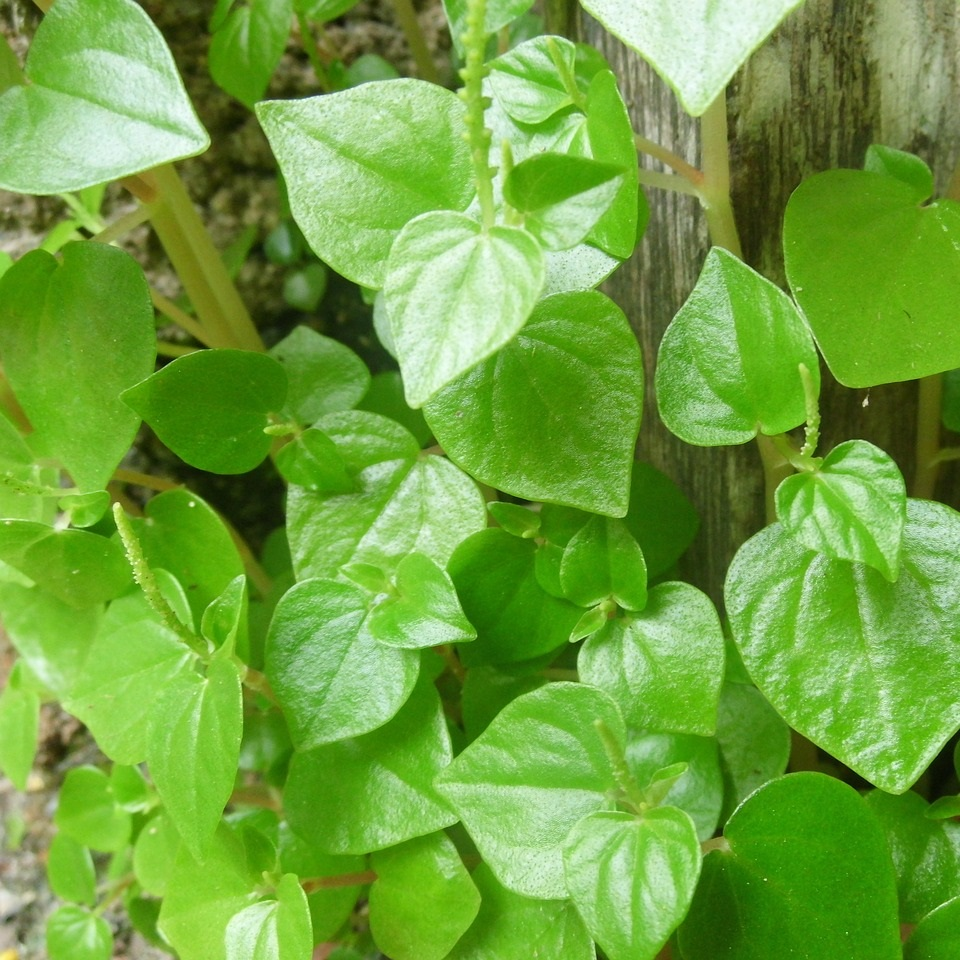
\includegraphics[width=\linewidth]{images/leafs.jpg}
\caption{Default Voronoi stipples generation}
\end{subfigure}%
\hfill
\begin{subfigure}[h]{0.4\linewidth}
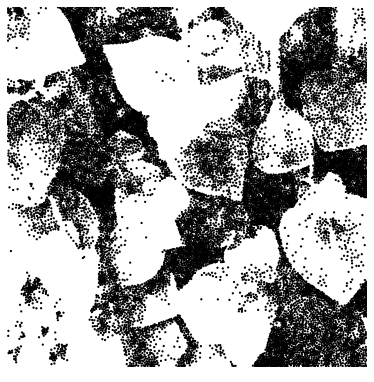
\includegraphics[width=\linewidth]{images/leafs_stippled.png}
\caption{Fast Voronoi stipples generation}
\end{subfigure}%
\caption{Examples of stippled images}
\label{comparison-fast}
\end{figure}

\subsubsection{Conclusion}
The resulting code offers similar results as shown in the original paper. The fast stippling method is assumed to be fast enough for real-time applications but unfortunately no test or comparison has been done. The results can be found in Github: https://github.com/FStoeltie/Vision

\subsubsection{Recommendations}
A few recommendations can be made for further study and improvements:


\begin{itemize}
  \item Section \nameref{precompute-stipple-levels} states that the results of the fast stippling method can be described as 'grainy' and comparable to the original distribution set. Developing a solution where these look more like the original Voronoi stippling method while keeping the complexity of \(O(n)\) for real-time applications might be worth researching. 
  \item The initial starting positions of points is the result of using an uniform distribution. By creating a custom function to generate points it is possible to add detail to certain parts - such as objects or contours. This might also result in more appealing images, especially for large and complex images multiple focal points. 
\end{itemize}